\documentclass[tikz,border=2pt]{standalone}
\usepackage{newtxtext,newtxmath}
\usepackage[T1]{fontenc}
\usetikzlibrary{arrows.meta,calc,positioning}

\definecolor{contextblue}{HTML}{2D72B8}
\definecolor{spanviolet}{HTML}{7251B5}
\definecolor{identifiergreen}{HTML}{2F7654}
\definecolor{warmborder}{HTML}{BC731D}
\definecolor{softgray}{HTML}{888888}

\begin{document}
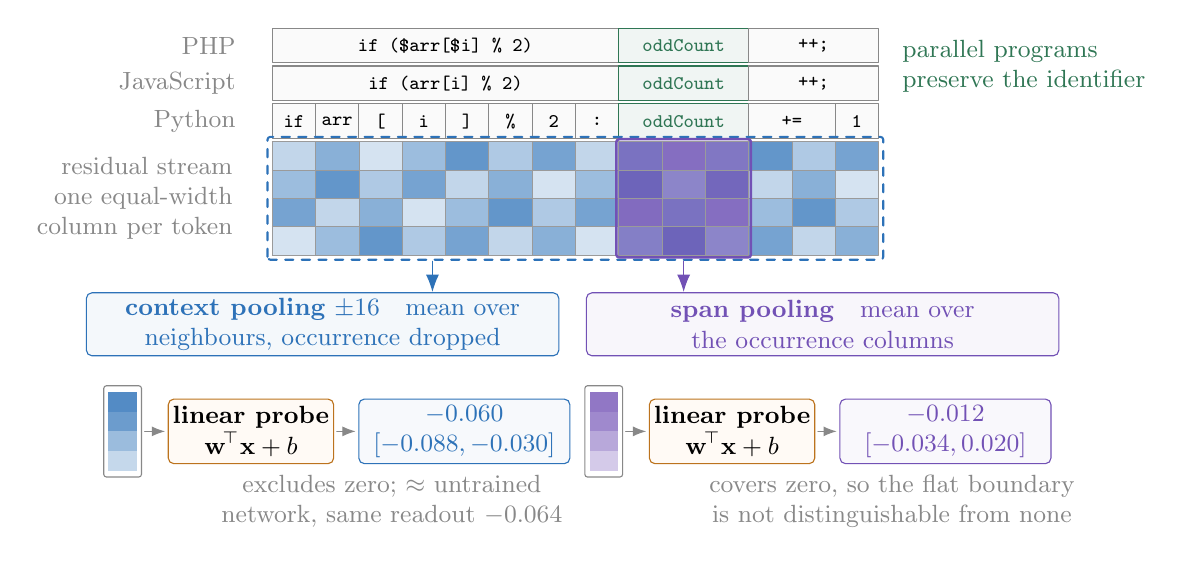
\begin{tikzpicture}[x=1cm,y=1cm,>=Latex,line cap=round,line join=round]
  \def\gx{2.78}
  \def\cw{0.55}
  \def\gh{0.36}
  \def\gridy{3.52}

  % Parallel source fragments. Every underlying slot has the same width.
  \foreach \lang/\yy in {PHP/6.18,JavaScript/5.70,Python/5.22}{
    \node[anchor=east,text=softgray,font=\small] at (2.44,\yy) {\lang};
  }
  \foreach \yy/\prefix/\suffix in {
    6.18/{if (\$arr[\$i] \% 2)}/{++;},
    5.70/{if (arr[i] \% 2)}/{++;}
  }{
    \draw[softgray,thin,fill=gray!4] (\gx,\yy-0.22) rectangle ({\gx+8*\cw},\yy+0.22);
    \draw[identifiergreen,thin,fill=identifiergreen!7] ({\gx+8*\cw},\yy-0.22)
      rectangle ({\gx+11*\cw},\yy+0.22);
    \draw[softgray,thin,fill=gray!4] ({\gx+11*\cw},\yy-0.22)
      rectangle ({\gx+14*\cw},\yy+0.22);
    \node[font=\ttfamily\scriptsize] at ({\gx+4*\cw},\yy) {\prefix};
    \node[text=identifiergreen,font=\ttfamily\scriptsize] at ({\gx+9.5*\cw},\yy) {oddCount};
    \node[font=\ttfamily\scriptsize] at ({\gx+12.5*\cw},\yy) {\suffix};
  }

  % Python makes the equal token slots explicit. The identifier is a span.
  \foreach \c/\tok in {0/if,1/arr,2/{[},3/i,4/{]},5/{\%},6/2,7/{:},13/1}{
    \draw[softgray,thin,fill=gray!4] ({\gx+\c*\cw},5.00)
      rectangle ({\gx+(\c+1)*\cw},5.44);
    \node[font=\ttfamily\scriptsize] at ({\gx+(\c+0.5)*\cw},5.22) {\tok};
  }
  \draw[identifiergreen,thin,fill=identifiergreen!7] ({\gx+8*\cw},5.00)
    rectangle ({\gx+11*\cw},5.44);
  \node[text=identifiergreen,font=\ttfamily\scriptsize] at ({\gx+9.5*\cw},5.22) {oddCount};
  \draw[softgray,thin,fill=gray!4] ({\gx+11*\cw},5.00)
    rectangle ({\gx+13*\cw},5.44);
  \node[font=\ttfamily\scriptsize] at ({\gx+12*\cw},5.22) {+=};

  \node[anchor=west,align=left,text=identifiergreen,font=\small]
    at ({\gx+14*\cw+0.18},5.92) {parallel programs\\preserve the identifier};

  % Residual stream: equal-width columns, one per schematic token slot.
  \foreach \r in {0,...,3}{
    \foreach \c in {0,...,13}{
      \pgfmathsetmacro{\op}{0.20+0.09*mod(3*\c+5*\r,7)}
      \fill[contextblue,fill opacity=\op]
        ({\gx+\c*\cw},{\gridy+\r*\gh})
        rectangle ({\gx+(\c+1)*\cw},{\gridy+(\r+1)*\gh});
    }
  }
  \foreach \r in {0,...,3}{
    \foreach \c in {8,...,10}{
      \pgfmathsetmacro{\op}{0.56+0.08*mod(2*\c+3*\r,4)}
      \fill[spanviolet,fill opacity=\op]
        ({\gx+\c*\cw},{\gridy+\r*\gh})
        rectangle ({\gx+(\c+1)*\cw},{\gridy+(\r+1)*\gh});
    }
  }
  % Draw each grid boundary once so every token column is visibly identical.
  \foreach \c in {0,...,14}{
    \draw[softgray!85,line width=0.24pt]
      ({\gx+\c*\cw},\gridy) -- ({\gx+\c*\cw},{\gridy+4*\gh});
  }
  \foreach \r in {0,...,4}{
    \draw[softgray!85,line width=0.24pt]
      (\gx,{\gridy+\r*\gh}) -- ({\gx+14*\cw},{\gridy+\r*\gh});
  }
  \draw[contextblue,dashed,line width=0.75pt,rounded corners=1pt]
    ({\gx-0.06},{\gridy-0.06}) rectangle
    ({\gx+14*\cw+0.06},{\gridy+4*\gh+0.06});
  \draw[spanviolet,line width=0.9pt,rounded corners=1pt]
    ({\gx+8*\cw-0.03},{\gridy-0.03}) rectangle
    ({\gx+11*\cw+0.03},{\gridy+4*\gh+0.03});

  \node[anchor=east,align=right,text=softgray,font=\small]
    at (2.40,{\gridy+2*\gh}) {residual stream\\one equal-width\\column per token};

  % Pooling rules.
  \draw[contextblue,-{Latex[length=2.2mm]},thin]
    ({\gx+3.7*\cw},\gridy-0.08) -- ({\gx+3.7*\cw},3.05);
  \draw[spanviolet,-{Latex[length=2.2mm]},thin]
    ({\gx+9.5*\cw},\gridy-0.08) -- ({\gx+9.5*\cw},3.05);

  \draw[contextblue,thin,rounded corners=2pt,fill=contextblue!5]
    (0.42,2.24) rectangle (6.42,3.04);
  \node[align=center,text=contextblue,font=\small] at (3.42,2.64)
    {\textbf{context pooling} $\pm16$\quad mean over\\neighbours, occurrence dropped};

  \draw[spanviolet,thin,rounded corners=2pt,fill=spanviolet!5]
    (6.77,2.24) rectangle (12.77,3.04);
  \node[align=center,text=spanviolet,font=\small] at (9.77,2.64)
    {\textbf{span pooling}\quad mean over\\the occurrence columns};

  % Readout and reported boundary for context pooling.
  \foreach \i/\op in {0/0.28,1/0.48,2/0.70,3/0.82}{
    \fill[contextblue,fill opacity=\op]
      (0.70,{0.78+\i*0.25}) rectangle (1.06,{1.03+\i*0.25});
  }
  \draw[softgray,thin,rounded corners=1pt]
    (0.64,0.70) rectangle (1.12,1.86);
  \draw[->,softgray] (1.16,1.28) -- (1.42,1.28);
  \draw[warmborder,thin,rounded corners=2pt,fill=orange!4]
    (1.46,0.87) rectangle (3.56,1.69);
  \node[font=\small,align=center] at (2.51,1.28)
    {\textbf{linear probe}\\$\mathbf{w}^{\!\top}\mathbf{x}+b$};
  \draw[->,softgray] (3.60,1.28) -- (3.84,1.28);
  \draw[contextblue,thin,rounded corners=2pt,fill=contextblue!4]
    (3.88,0.87) rectangle (6.56,1.69);
  \node[text=contextblue,font=\small,align=center] at (5.22,1.28)
    {$-0.060$\\$[-0.088,-0.030]$};
  \node[align=center,text=softgray,font=\small] at (4.30,0.39)
    {excludes zero; $\approx$ untrained\\network, same readout $-0.064$};

  % Readout and reported boundary for span pooling.
  \foreach \i/\op in {0/0.30,1/0.50,2/0.68,3/0.78}{
    \fill[spanviolet,fill opacity=\op]
      (6.81,{0.78+\i*0.25}) rectangle (7.17,{1.03+\i*0.25});
  }
  \draw[softgray,thin,rounded corners=1pt]
    (6.75,0.70) rectangle (7.23,1.86);
  \draw[->,softgray] (7.27,1.28) -- (7.53,1.28);
  \draw[warmborder,thin,rounded corners=2pt,fill=orange!4]
    (7.57,0.87) rectangle (9.67,1.69);
  \node[font=\small,align=center] at (8.62,1.28)
    {\textbf{linear probe}\\$\mathbf{w}^{\!\top}\mathbf{x}+b$};
  \draw[->,softgray] (9.71,1.28) -- (9.95,1.28);
  \draw[spanviolet,thin,rounded corners=2pt,fill=spanviolet!4]
    (9.99,0.87) rectangle (12.67,1.69);
  \node[text=spanviolet,font=\small,align=center] at (11.33,1.28)
    {$-0.012$\\$[-0.034,0.020]$};
  \node[align=center,text=softgray,font=\small] at (10.65,0.39)
    {covers zero, so the flat boundary\\is not distinguishable from none};
\end{tikzpicture}
\end{document}
